Questo elaborato descrive il lavoro di tirocinio e tesi svolto presso il CNAF
(Centro Nazionale delle Tecnologie Informatiche e Telematiche) dell'INFN
(Istituto Nazionale di Fisica Nucleare), uno dei più importanti centri di
calcolo in Italia. Questo centro processa e gestisce decine di petabyte di
dati. L'obiettivo è stato quello di analizzare questi dati per identificare un
problema che potesse essere risolto tramite l'uso di tecniche di Machine
Learning e Deep Learning.

In questo capitolo forniremo una panoramica del centro di calcolo, guardando
da dove provengono i dati e come vengono raccolti. Verrà infine presentato il
problema che è stato oggetto della nostra analisi, spiegando le motivazioni
alla base di questa scelta.

\section{Il cluster di calcolo del CNAF}

Il \textbf{Grid computing} è un'architettura di calcolo distribuito che
collega centri di calcolo sparsi geograficamente allo scopo di condividere
risorse e potenza di calcolo per raggiungere uno scopo condiviso. Attualmente,
il più grande sistema Grid al mondo è il Worldwide LHC Computing Grid (WLCG),
che nasce da una collaborazione internazionale che coinvolge oltre 170 centri
di calcolo sparsi in più di 40 nazioni. Lo scopo del WLCG è fornire
l'infrastruttura computazionale necessaria per gestire i dati generati dagli
esperimenti di Fisica delle Alte Energie effettuati con il Large Hadron
Collider (LHC) \cite{WLCG2023}.

Come illustrato nella figura~\ref{fig:WLCG_tier_hierarchy}, i centri di
calcolo all'interno del WLCG sono strutturati secondo il modello MONARC, che
li organizza in un sistema gerarchico di livelli, noti come Tier, ciascuno dei
quali ha funzioni e responsabilità ben definite. In questo contesto si colloca
il CNAF, che ospita il Tier-1 per tutti e quattro gli esperimenti del LHC.
Oltre a questi ultimi, vengono supportati presso il CNAF anche alcuni
esperimenti non-LHC di astrofisica delle particelle e fisica dei neutrini
\cite{Bortolotti2012}.

\begin{figure}[ht]
    \centering
    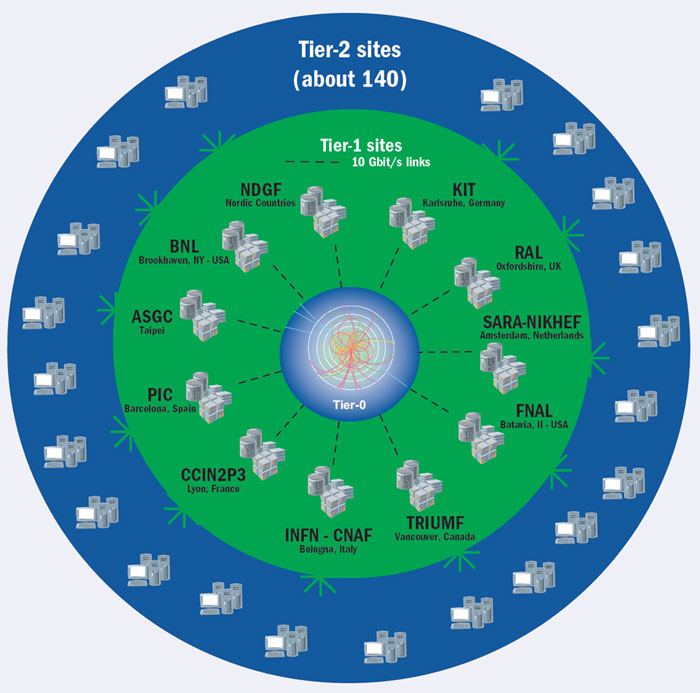
\includegraphics[width=0.75\linewidth]{WLCG_tier_hierarchy}
    \caption{Struttura gerarchica del WLCG \protect\cite{dalpra2019}}
    \label{fig:WLCG_tier_hierarchy}
\end{figure}

Il CNAF offre più di 46000 core distribuiti su 960 host fisici per un totale
di circa $630$ kHS06 di potenza di calcolo \cite{hepix2022}. L'allocazione di
queste risorse segue il paradigma del \textbf{High-Throughput Computing}
(HTC), dove a differenza dell'High-Performance Computing, che mira a ridurre
il wall-clock time dei programmi, HTC mira a massimizzare il throughput,
intenso come il numero di job completati per unità di tempo.

In questo sistema, gli utenti sono raggruppati in circa 50 gruppi distinti,
ciascuno dei quali corrisponde a un esperimento scientifico specifico. A ogni
gruppo è assegnata una quota di risorse che può utilizzare. Quando un utente
ha bisogno di utilizzare queste risorse, può sottomettere un \textbf{job} al
sistema, che rappresenta una o più operazioni computazionali.

Una volta sottomesso, il job non viene eseguito immediatamente, ma viene messo
in una coda gestita da un batch system (HTCondor). Quest'ultimo è responsabile
della schedulazione dei job in coda, decidendo quale job eseguire, quando e
dove. Per farlo, utilizza algoritmi di ``fairshare'', che sono pensati per
assicurare una distribuzione equa delle risorse computazionali disponibili,
impedendo che un singolo utente o un intero gruppo possa monopolizzare tutte
le risorse disponibili.

%Una volta sottomesso, il job non viene eseguito immediatamente, ma viene messo
%in una coda gestita da un batch system (HTCondor). Quest'ultimo è responsabile
%della schedulazione dei job in coda, decidendo quale job eseguire, quando e
%dove. Per farlo, utilizza algoritmi di ``fairshare'', che sono pensati per
%assicurare una distribuzione equa delle risorse computazionali disponibili. Il
%fairshare previene due fenomeni indesiderati: in primo luogo, la starvation,
%ossia situazioni in cui i job a bassa priorità non vengono mai eseguiti perché
%continuativamente ``scavalcati'' da job più prioritari; in secondo luogo,
%l'underusage, cioè il rischio di avere CPU inutilizzate in momenti in cui
%alcuni gruppi non stanno utilizzando le risorse, cosa che si verificherebbe
%con un partizionamento statico delle risorse di calcolo.

Se un gruppo non utilizza la quota di risorse assegnata, queste vengono
redistribuite tra i gruppi attivi in proporzione alla loro quota. Questo
meccanismo assicura che la farm di calcolo lavori quasi sempre alla sua
massima capacità, ottimizzando l'uso delle risorse nel lungo termine
\cite{cnaf_calcolo}.

\section{La base di dati}

Il caso di studio di questa tesi si basa su informazioni provenienti da due
fonti principali: la prima è ottenuta attraverso il monitoraggio dello stato
dei job in esecuzione, effettuato tramite il comando \texttt{condor\_q} di
HTCondor, eseguito ogni 3 minuti. La seconda proviene dai file
\textit{history}, generati automaticamente da HTCondor al termine
dell'esecuzione di ciascun job e che rappresentano lo stato finale dei job.

Successivamente uno script estrae le informazioni rilevanti dai dati di
accounting; queste informazioni vengono poi inserite nella tabella
\texttt{htjob} di un database PostgresSQL. Analogamente, i dati di
monitoraggio vengono raccolti e caricati su una tabella \texttt{hj}.

La raccolta dei dati è stata effettuata in due periodi distinti: il primo da
settembre a dicembre 2021, e il secondo nel mese di marzo 2023. I dati sono
stati immagazzinati in due database separati, identificati come \texttt{htm}
per i dati del primo periodo e \texttt{htmnew} per quelli del secondo.

\begin{table}[!htbp]
    \centering 
    \begin{tabular}{
      lrr
    }
        \toprule 
        & \multicolumn{2}{c}{\textbf{htm}} \\
        \cmidrule{2-3}
        & {\textbf{Righe}} & {\textbf{Spazio (GB)}} \\ 
        \midrule
        \texttt{hj}      & 1971830783 & 343 \\
        \texttt{htjob}   & 30799153 & 14 \\
        \bottomrule
    \end{tabular}
    \hspace*{1cm}
    \begin{tabular}{lrr}
        \toprule
        & \multicolumn{2}{c}{\textbf{htmnew}} \\
        \cmidrule{2-3}
        & {\textbf{Righe}} & {\textbf{Spazio (GB)}} \\
        \midrule
        \texttt{hj}      & 1038471316 & 222 \\
        \texttt{htjob}   & 46605815 & 22 \\
        \bottomrule
    \end{tabular}
    \caption{Confronto delle dimensioni tra i database \texttt{htm} e \texttt{htmnew}}
    \label{table:database_comparison}
\end{table}

\begin{table}[p]
    \centering
    \caption{Schema della tabella \texttt{hj} del database}
    \begin{tabular}{llp{6cm}}
        \toprule
        \textbf{Colonna} & \textbf{Tipo} & \textbf{Descrizione} \\
        \midrule
        \texttt{ts} & Numerico (secondi) & Timestamp UNIX del momento in
        cui lo stato del job viene misurato \\
        \texttt{jobid + idx} & Categorico (Nominale) & ID univoco del job \\
        \texttt{queue}  & Categorico (Nominale) & Gruppo di appartenenza
        dell'utente che ha sottomesso il job \\
        \texttt{hn (hostname)} & Categorico (Nominale) & Host sul quale il job è in esecuzione \\
        \texttt{js} & Categorico (Nominale) & Stato del job: 1 = In coda, 2 = In esecuzione, 3 = Rimosso, 4 = Completato, 5 = Sospeso \\
        \texttt{nc} & Numerico (core) & Numero di core CPU impiegati dal job \\
        \texttt{hsj} & Numerico (HS06) & Potenza di un core del host \\
        \texttt{hsm} & Numerico (HS06) & Potenza totale del host \\
        \texttt{cpt (cputime)} & Numerico (secondi) & Tempo di esecuzione sulla CPU del job\\
        \texttt{rt (runtime)} & Numerico (secondi) & Tempo totale di esecuzione del job\\
        \texttt{owner} & Testo & Utente che ha sottomesso il job (username UNIX) \\
        \texttt{rss} & Numerico (KB) & Memoria RAM utilizzata
        dal job\\
        \texttt{swp} & Numerico (KB) & Memoria SWAP utilizzata
        dal job\\
        \texttt{sn (submitnode)} & Categorico (Nominale) & Nodo da cui è stato sottomesso il job \\
        \texttt{disk} & Numerico (GB) & Spazio su disco
        utilizzato dal job \\
        \bottomrule
    \end{tabular}
    \label{table:schema_hj}
\end{table}

\begin{table}[p]
  \centering
  \caption{Schema della tabella \texttt{htjob} del database}
  \footnotesize
  \begin{tabular}{llp{6cm}}
    \toprule
    \textbf{Colonna} & \textbf{Tipo} & \textbf{Descrizione} \\
    \midrule
    \texttt{jobid + idx} & Categorico (Nominale) & ID univoco del job \\
    \texttt{username} & Testo & Utente che ha sottomesso il job (username UNIX) \\
    \texttt{queue} & Categorico (Nominale) & Gruppo di appartenenza dell'utente che ha sottomesso il
    job \\
    \texttt{fromhost} & Categorico (Nominale) & Nodo da cui è stato sottomesso il job \\
    \texttt{jobname} & Testo & Nome del job \\
    \texttt{exechosts} & Categorico (Nominale) & Host sul quale il job è in esecuzione \\
    \texttt{submittimeepoch} & Numerico (secondi) & Timestamp UNIX del momento in cui il
    job è stato sottomesso \\
    \texttt{starttimeepoch} & Numerico (secondi) & Timestamp UNIX del momento in cui il
    job è stato eseguito \\
    \texttt{eventtimeepoch} & Numerico (secondi) & Timestamp UNIX del momento in cui il
    job è terminato \\
    \texttt{stime} & Numerico (secondi) & Tempo di esecuzione sulla CPU per
    eseguire le chiamate al sistema per conto del job \\
    \texttt{utime} & Numerico (secondi) & Tempo di esecuzione sulla CPU
    dedicato alle operazione che il job esegue direttamente \\
    \texttt{runtime} & Numerico (secondi) & Tempo totale di esecuzione del job \\
    \texttt{maxrmem} & Numerico (KB) & Massima memoria RAM utilizzata dal job \\
    \texttt{maxrswap} & Numerico (KB) & Massima memoria SWAP utilizzata dal job \\
    \texttt{exitstatus} & Categorico (Nominale) & = 0 è ok; != 0 è uscito con errore \\
    \texttt{numprocessors} & Numerico (core) & Numero di core CPU impiegati dal job \\
    \texttt{gpu} & Categorico (Nominale) & 1 = gpu utilizzata; 0 = gpu non utilizzata \\
    \texttt{completionepoch} & Numerico (secondi) & Timestamp UNIX del momento in cui il
    job è terminato \\
    \texttt{jobstatus} & Categorico (Nominale) & Stato del job: 1 = In coda, 2 = In esecuzione, 3 = Rimosso, 4 = Completato, 5 = Sospeso \\
    \bottomrule
  \end{tabular}
  \label{table:schema_htjob}
\end{table}

La tabella~\ref{table:database_comparison} mostra il numero totale di righe e
lo spazio occupato su disco da ciascuna tabella nei database. Dato che la
dimensione del dataset supera la capacità della memoria RAM a disposizione,
risulta impossibile analizzare l'intero dataset. Pertanto, diventa necessario
selezionare un sottoinsieme di dati da tali database per effettuare le analisi
successive.

Le tabelle \ref{table:schema_hj} e \ref{table:schema_htjob} offrono una
panoramica sulle colonne presenti, distinguendo tra variabili categoriche e
numeriche e fornendo una breve spiegazione su ciascuna colonna. 

Le variabili si suddividono in base al tipo di dati che rappresentano e si
suddividono in: 

\begin{itemize}
    \item \textit{categorico nominale}, se contiene valori scelti tra un
        insieme finito;
    \item \textit{categorico ordinale}, è simile, ma si definisce una
        relazione d'ordine tra i valori possibili;
    \item \textit{numerico}, se è possibile quantificare le differenze tra valori.
\end{itemize}

\section{Motivazione}

Nel 1965, Gordon Moore, co-fondatore di Intel, pronosticò che il numero di
transistor sarebbe raddoppiato ogni 18 mesi \cite{Moore1965}. Tuttavia, il
trend descritto da Moore arriverà a un termine quando la litografia, il
processo usato per stampare i circuiti sui wafer di silicio, raggiungerà la
scala atomica. Infatti, a scale atomiche i transistor incontrano fenomeni
quantistici che ne disturbano il funzionamento, e le attuali tecniche di
produzione diventano proibitive in termine di costi \cite{Shalf2015,
Theis2017}.

I sistemi HTC e HPC sono divenuti strumenti fondamentali per il progresso
della ricerca scientifica. Nonostante ciò, vi sono ancora molteplici problemi
importanti in vari settori che non possono essere risolti con le capacità
computazionali attuali \cite{Villa2014}. Per proseguire l'evoluzione
tecnologica nell'era post-legge di Moore è quindi necessario esplorare nuove
direzioni. Una di queste riguarda l'incremento del numero di core.

In questa tesi, un \textit{guasto} è definito come un comportamento anomalo a
livello software o hardware, che può causare stati illeciti (\textit{errori})
nel sistema o nell'applicazione e che, nel peggiore dei casi, può causarne
l'interruzione (\textit{fallimenti}).

Sfortunatamente, più core si aggiungono, maggiori sono le probabilità di
riscontrare guasti hardware. In parallelo, all'aumentare della complessità
hardware, si assiste a una crescente complessità del software, il che lo rende
più suscettibile agli errori \cite{Cappello2014}.

\begin{figure}[!ht]
    \begin{center}
        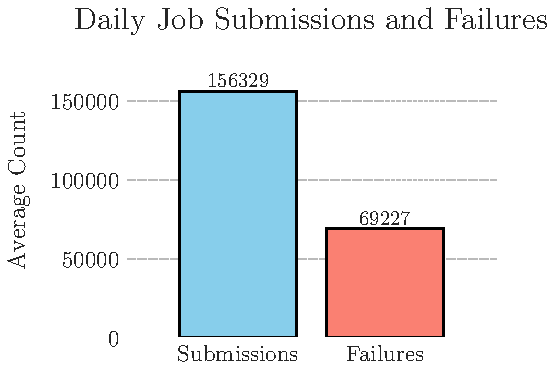
\includegraphics[width=0.5\linewidth]{daily_job_submissions_and_failures}
    \end{center}
    \caption{Media giornaliera di job sottomessi e falliti nel mese di Marzo
    2023}\label{fig:daily_job_submissions_and_failures}
\end{figure}

Come evidenziato nella figura~\ref{fig:daily_job_submissions_and_failures}, si
osserva che in un centro di calcolo come quello del CNAF, nel mese di Marzo
2023, sono stati sottomessi giornalmente in media circa 150000 job con un
tasso di fallimento che supera il 40\%. 
La frequenza con cui i job falliscono rappresenta una problematica
significativa per i centri di calcolo: questa non solo causa uno spreco delle
risorse del sistema, ma incide anche negativamente sull'efficienza generale e
allunga i tempi d'attesa per i job in coda.

Questa tesi si concentra sui fallimenti dei job piuttosto che sui fallimenti a
livello di sistema, nonostante la disponibilità di dati degli host fisici del
CNAF. Utilizzando tecniche di Machine Learning per identificare pattern nei
dati storici, potrebbe essere possibile prevedere la riuscita o il fallimento
di un job basandosi sul comportamento di job simili. Questo permetterebbe
l'adozione di strategie proattive volte a prevenire i fallimenti prima che
accadano, mitigando così i problemi sopracitati. In aggiunta, la capacità di
informare l'utente circa il tasso di successo o fallimento di un job che sta
per essere sottomesso potrebbe fornire una risorsa informativa utile.

\mbox{}

Nel capitolo~\ref{chap:analisi}, si descrive come l'analisi preliminare abbia
evidenziato una categoria di job che falliscono, che risulta essere
particolarmente interessante, soprattutto per l'importanza di identificarli e
rimuoverli tempestivamente.

\mbox{}

Nel capitolo~\ref{chap:teoria}, si tratta dell'estrazione e della preparazione
dei dati per l'addestramento di modelli predittivi. In seguito, si esplorano i
modelli specifici per due modellazioni diverse del problema di identificazione
di questa categoria di job.

\mbox{}

Nel capitolo~\ref{chap:applicazione}, si introduce inizialmente una
metodologia per valutare correttamente i risultati ottenuti. Successivamente,
si discutono i risultati derivanti dall'applicazione dei modelli, illustrando
due approcci differenti utilizzati.

\mbox{}

Nel capitolo~\ref{chap:conclusione}, si fornisce una sintesi dei risultati
raggiunti e si propongono potenziali direzioni per ulteriori sviluppi e
miglioramenti. 
